% main.tex
% Compile with LuaLaTeX (recommended) or XeLaTeX
\documentclass[%
    colorscheme=blue,   % Options: default, green, blue, red, purple
    fontsize=36pt,        % Options: 36pt, 42pt, 48pt, ...
    papersize=a0paper,    % Options: a0paper, a1paper, a2paper, a3paper, a4paper, letterpaper, ...
    paper=930mm:1000mm,
    orientation=portrait, % Options: portrait, landscape
    debug=false           % Options: true, false
]{betterposterv2}

\usepackage{kotex}
\usepackage{listings}
\pdfpkresolution=300
% --- Poster Layout (optional overrides) ---
% Customize poster geometry (defaults shown):
\SetHeaderHeight{7cm}
\SetFooterHeight{6cm}
\SetSideMargin{2cm}

% --- Color Customization (optional) ---
% Override individual colors (defaults use colorscheme option):
% \SetPageColor{bpLightGrey}
% \SetHeaderColor{bpDark}
% \SetFooterColor{bpDark}
% \SetLightBoxColor{bpWhite}
% \SetDarkBoxColor{bpMediumGrey}
% \SetHeaderTextColor{white}
% \SetFooterTextColor{white}

% --- Font Size Customization (optional) ---
% Customize font sizes (defaults shown):
% \SetMainFindingSize{\Huge}
% \SetTitleSize{\Large}
% \SetBoxTitleSize{\large}
% \SetSectionSize{\Large}

% --- Poster Content Configuration ---
% Your main finding - This is the most important message of your poster
\SetMainFindingSize{\Large}
\mainfinding{TraceInspector - 추적 가능한 시각화 기반 코드 정적분석기}

% Your poster title
% \title{요약해석을 활용한 코드 정적분석 및 시각화}
\title{}

% --- Footer Configuration ---
% QR code to your project/website (optional - comment out if not needed)
% \qrcode{example-image}
% QR code label/subtitle (optional - appears below QR code)
% \qrcodelabel{\href{https://example.org}{example.org}}  % Or a simple: Scan me!
% Authors - use \textsuperscript{} for affiliation markers if needed
\authors{20212978 김신영, 20212952 강민성}
% Affiliations - can use line breaks with \\
\affiliations{국민대학교 소프트웨어학부}
% Institution logo (optional)
\logo{images/symbol_color.jpg}
% Publication year
% \publicationyear{2026}
% Author portrait/photo (optional - comment out if not needed)
% \portrait{example-image}

\begin{document}

\maketitle
\newcommand{\inleq}[1]{\scalebox{1.7}{$#1$}}
% --- BLOCK 1: BACKGROUND (Wide Grey Box) ---
% Use bpcolor=grey for darker background, bpstyle=wide for full-width
% Use bptitle=transparent to make title background blend with page
\begin{bpbox}[bpcolor=grey, bpstyle=wide, title={배경}]
    정적 분석(Static Analysis)은 프로그램을 실행하지 않고 코드의 실행 특성을 추론하여 잠재적인 오류를 탐지하는 기술이다.
    IDE, 컴파일러, CI 환경 등 다양한 개발 과정에서 코드 품질과 안정성을 높이기 위해 널리 활용되고 있음.

    기존 분석기들은 분석 결과만 제시할 뿐 왜 발생했는지 이해하기 어렵고, 분석 과정을 일종의 “블랙박스”처럼 받아들이고 결과를 맹신하게 됨.
\end{bpbox}

\begin{bpbox}[title={TraceInspector 소개}]
    TraceInspector는 요약해석(Abstract Interpretation) 이론을 바탕으로 한 정적 분석기와 더불어 분석 과정을 시각적으로 보여주는 인터페이스로 구성되어 있음.

    분석 중 생성되는 요약 상태(Abstract State)의 변화 과정을 사용자에게 실시간으로 보여주어 각 프로그램 지점에서 정보가 어떻게 전파 및 정제되는지를 직관적으로 관찰할 수 있도록 구현함.
\end{bpbox}

\bpsection{\textbf{분석 과정}}

% --- BLOCK 2: TWO-COLUMN SECTION ---
% Section headers align with box titles
% \bpsection{Results}
% Use bpcolumns[2] for 2 columns, bpcolumns[3] for 3 columns, etc.
\begin{bpcolumns}[3]
    % Left column box
    \begin{bpbox}[title={1: Go 코드 \inleq{\rightarrow} 중간 표현 언어(\inleq{\mathsf{Imp}})}, bptitlebg=transparent]  % Titlebg can be made transparent
        Go AST를 간단한 형태의 \inleq{\mathsf{Imp}} 언어로 번역. 분석기는 \inleq{\mathsf{Imp}} 코드에 대해 동작하며, 분석기 구현 및 타 언어 이식 시 용이하도록 설계.

        % Example of including a figure with caption
        \begin{center}
            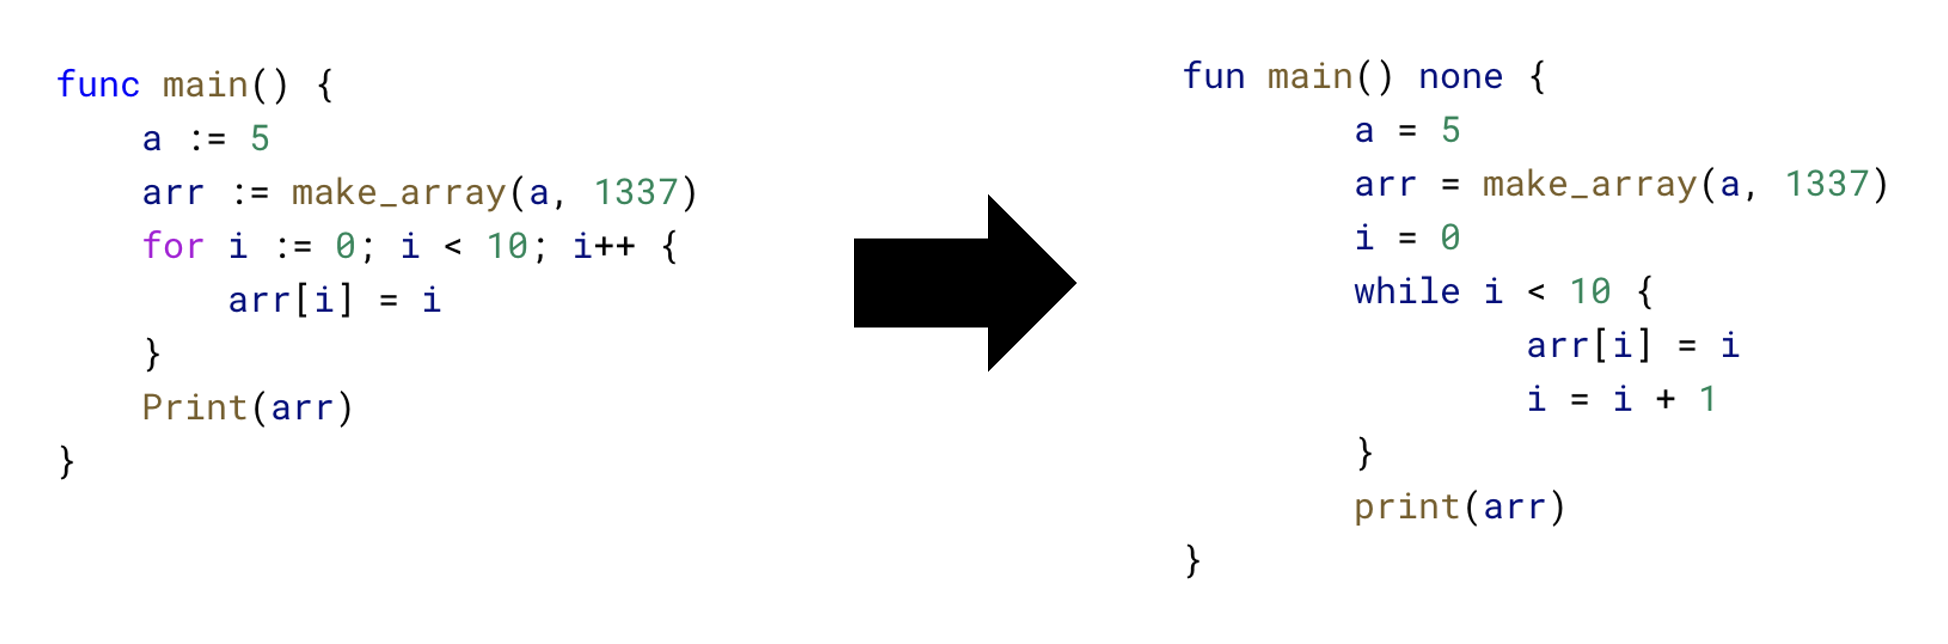
\includegraphics[width=\linewidth, height=11cm, keepaspectratio]{images/go2imp.png}%
        \end{center}
    \end{bpbox}
    % Right column box, make sure theres no empty line between boxes! 
    \begin{bpbox}[bptitlebg=transparent, title={2: \inleq{\displaystyle \mathsf{Imp} \rightarrow} 제어 흐름 그래프(CFG)}]  % Titlebg can be made transparent
        프로그램 내 분기, 반복 등의 제어 흐름 단위로 나타내는 제어 흐름 그래프 형태로 표현. 각각의 명령문들은 단일 노드로 표현됨.

        \begin{center}
            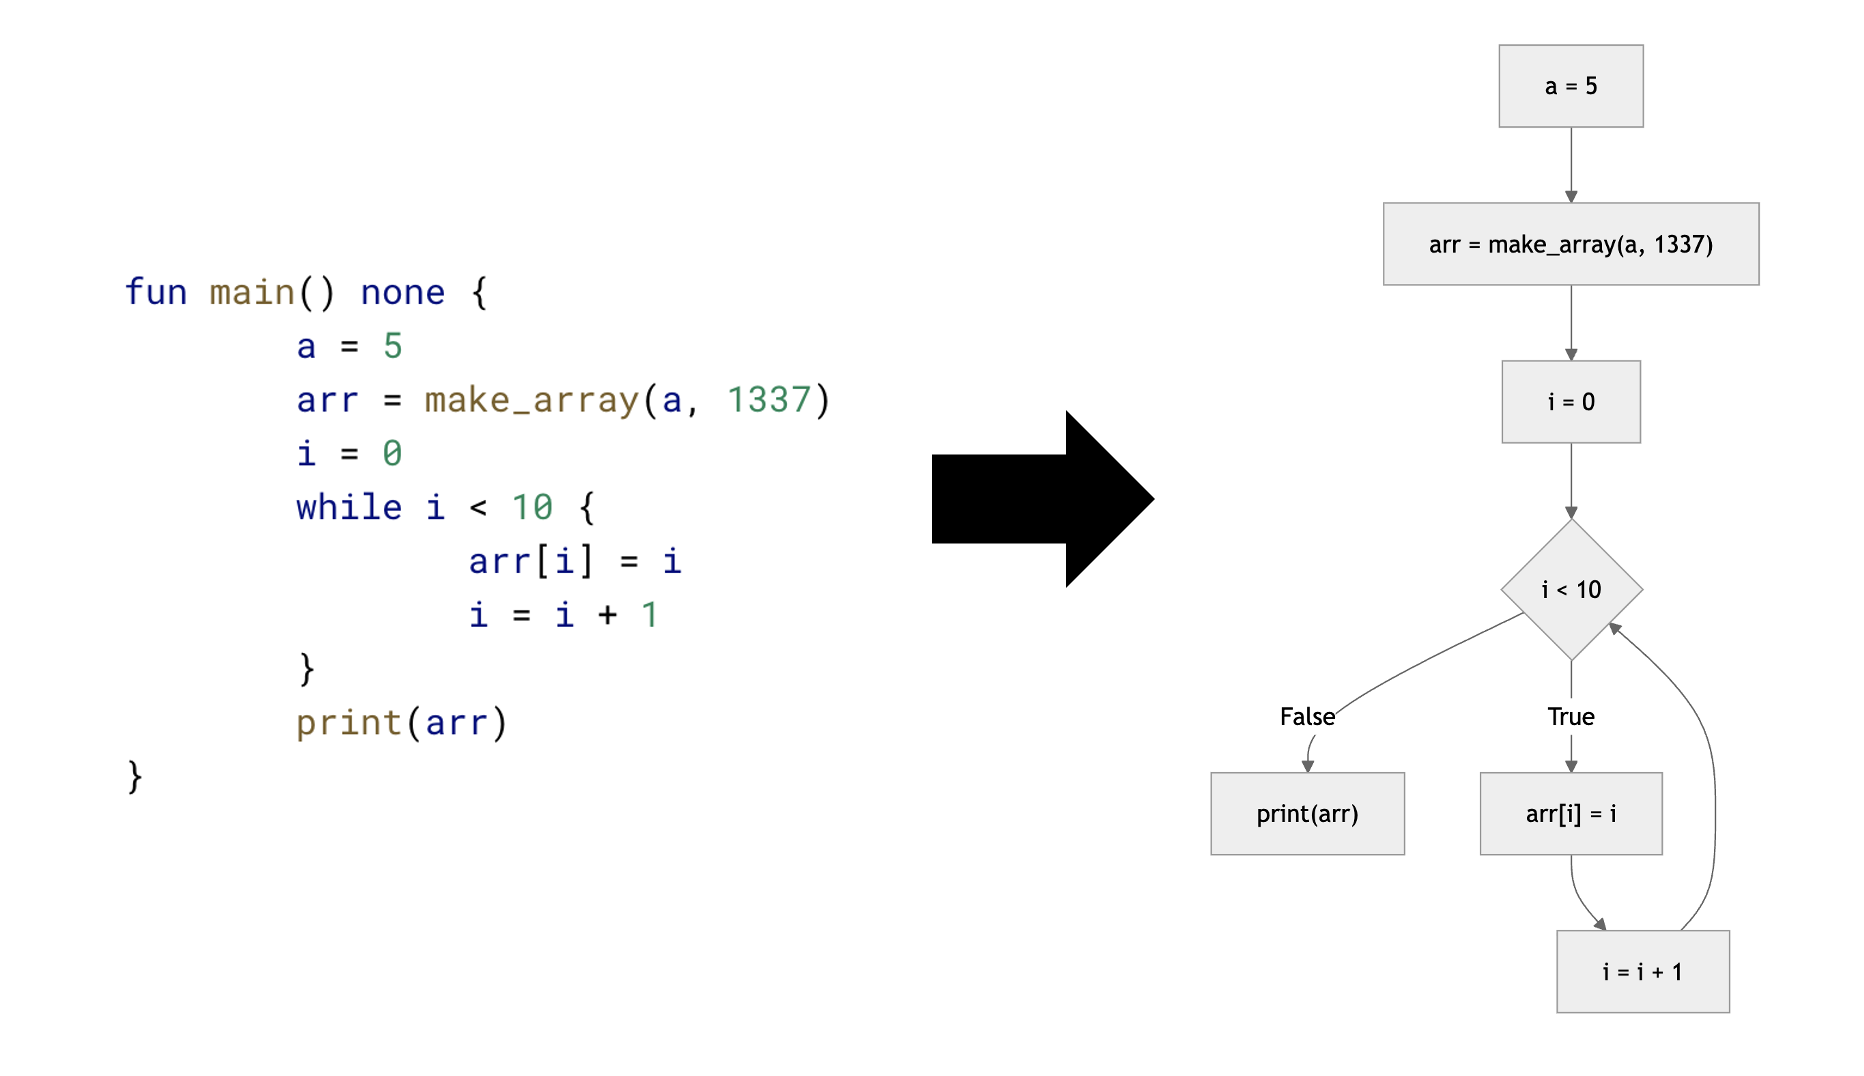
\includegraphics[width=\linewidth, height=11cm, keepaspectratio]{images/imp2cfg.png}%
        \end{center}
    \end{bpbox}
    \begin{bpbox}[bptitlebg=transparent, title={3: CFG 위에서 고정점 근사}]
        CFG 노드별 진입 시점에서의 프로그램 상태를 근사. 고정점에 도달할 때까지 반복적으로 요약실행 및 상태 join/widening 수행.

        \begin{center}
            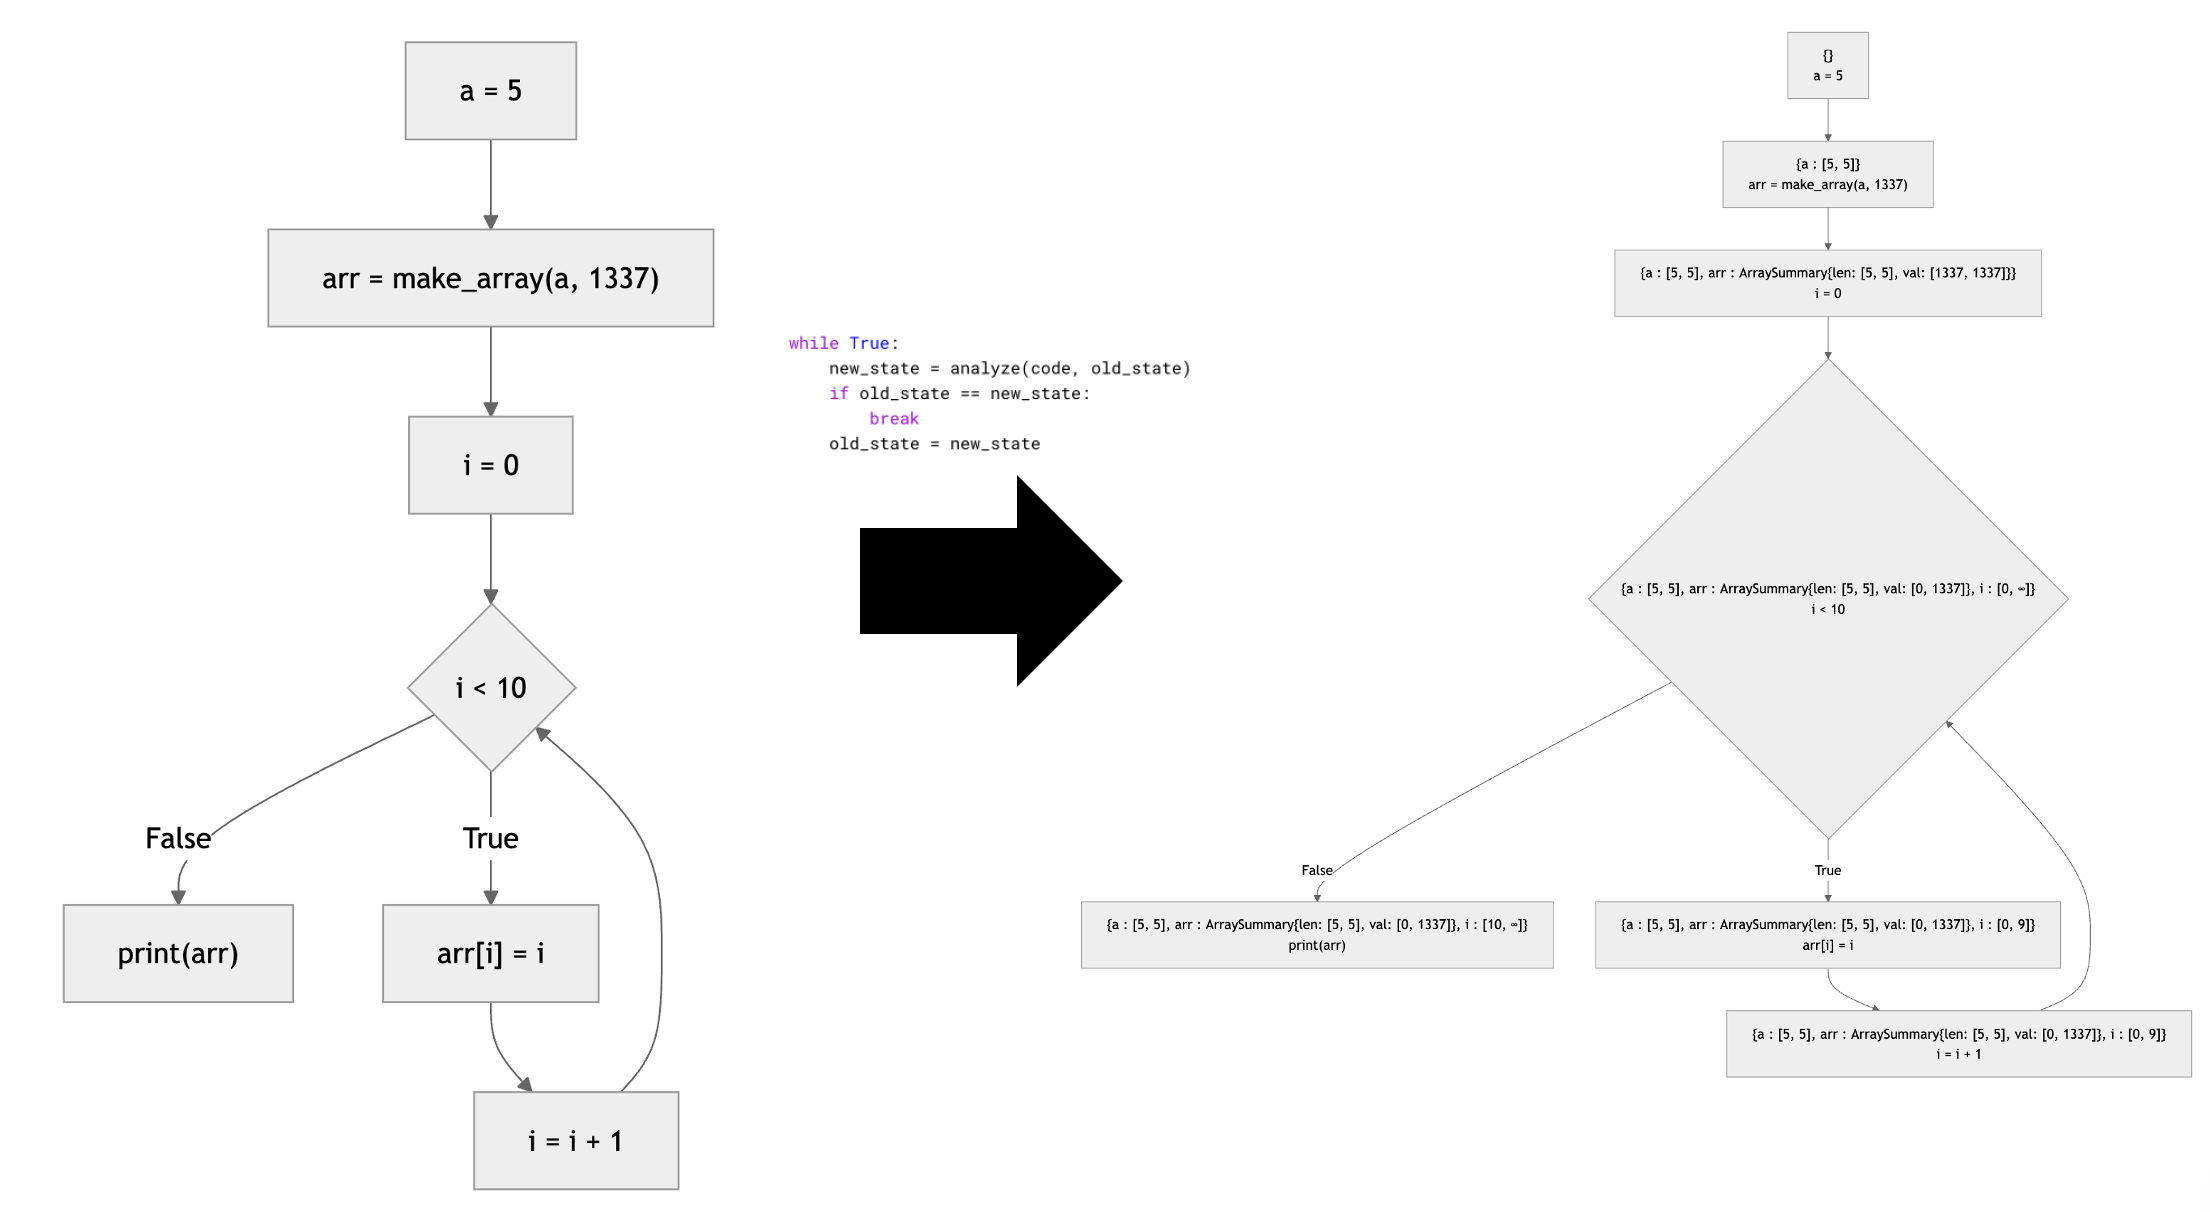
\includegraphics[width=\linewidth, height=11cm, keepaspectratio]{images/cfg2fixpoint.png}%
        \end{center}
    \end{bpbox}
\end{bpcolumns}

% --- BLOCK 3: Methods ---
\begin{bpcolumns}[2]
    \begin{bpbox}[title={분석 예시: 무한 루프}, bptitlebg=transparent]
        \noindent
        \begin{minipage}{0.5\textwidth}
            \begin{lstlisting}[language=Go, numbers=left, mathescape, xleftmargin=0.5cm]
func main() {
    a := 1       a: [1, 1]
    for a > 0 {  a: [1, 5]
        a++      a: [1, $\infty$]
    }            a: $\bot$
    Print(a)     a: $\bot$
}
            \end{lstlisting}
        \end{minipage}
        \vline \hfill
        \begin{minipage}{0.45\textwidth}
            \vspace{-0.7\baselineskip}
            무한히 반복되는 코드의 경우 \inleq{n}번의 몸통 실행 후, 계산된 상태에 대해 widening 기법을 적용하여 분석이 종료할 수 있도록 유도.
            이후 flitering을 통해 widening 결과를 정제하여 정확도 손실을 방지함. 
        \end{minipage}
    \end{bpbox}
    \begin{bpbox}[title={분석 예시: 배열 인덱싱 범위}, bptitlebg=transparent]
        \begin{lstlisting}[language=Go, numbers=left, mathescape, xleftmargin=0.5cm]
i := 1                i: [1, 1]
for i < len(arr) {    i: [1, 10], len(arr): [10, 10]
    key := arr[i]     i: [1, 9]
    arr[i+1] = arr[i] i: [1, 9], key: [0, 10]
Print(i)              i: [10, 10], key: [0, 10]
        \end{lstlisting}
        \hrule \kern15pt
        배열의 길이와 인덱스 변수에 대한 요약상태를 계산 후, 안전한 인덱싱 범위인지 확인함. 
    \end{bpbox}
\end{bpcolumns}

% Standard white box (default)
% \begin{bpbox}[title={}]  % Title can be omitted as well, which removes the title bar
%     % Example of side-by-side content using minipages
%     \begin{minipage}{0.45\textwidth}
%         Lorem ipsum dolor sit amet, consectetur adipiscing elit. Sed do eiusmod tempor incididunt ut labore et dolore magna aliqua. Ut enim ad minim veniam, quis nostrud exercitation ullamco laboris.

%         % Example of using siunitx for units
%         The measured value was \SI{42.5}{\milli\meter} with an uncertainty of \SI{0.5}{\milli\meter}.
%     \end{minipage}%
%     \hfill
%     \begin{minipage}{0.5\textwidth}
%         \centering
%         \includegraphics[width=\linewidth,height=6cm, keepaspectratio]{example-image-b}%
%         \captionof{figure}{Results visualization}
%     \end{minipage}
% \end{bpbox}

\begin{bpcolumns}[2]
    \begin{bpbox}[bpcolor=grey, bpstyle=wide, title={시각화}]
        \begin{minipage}{0.7\textwidth}
            \begin{center}
                    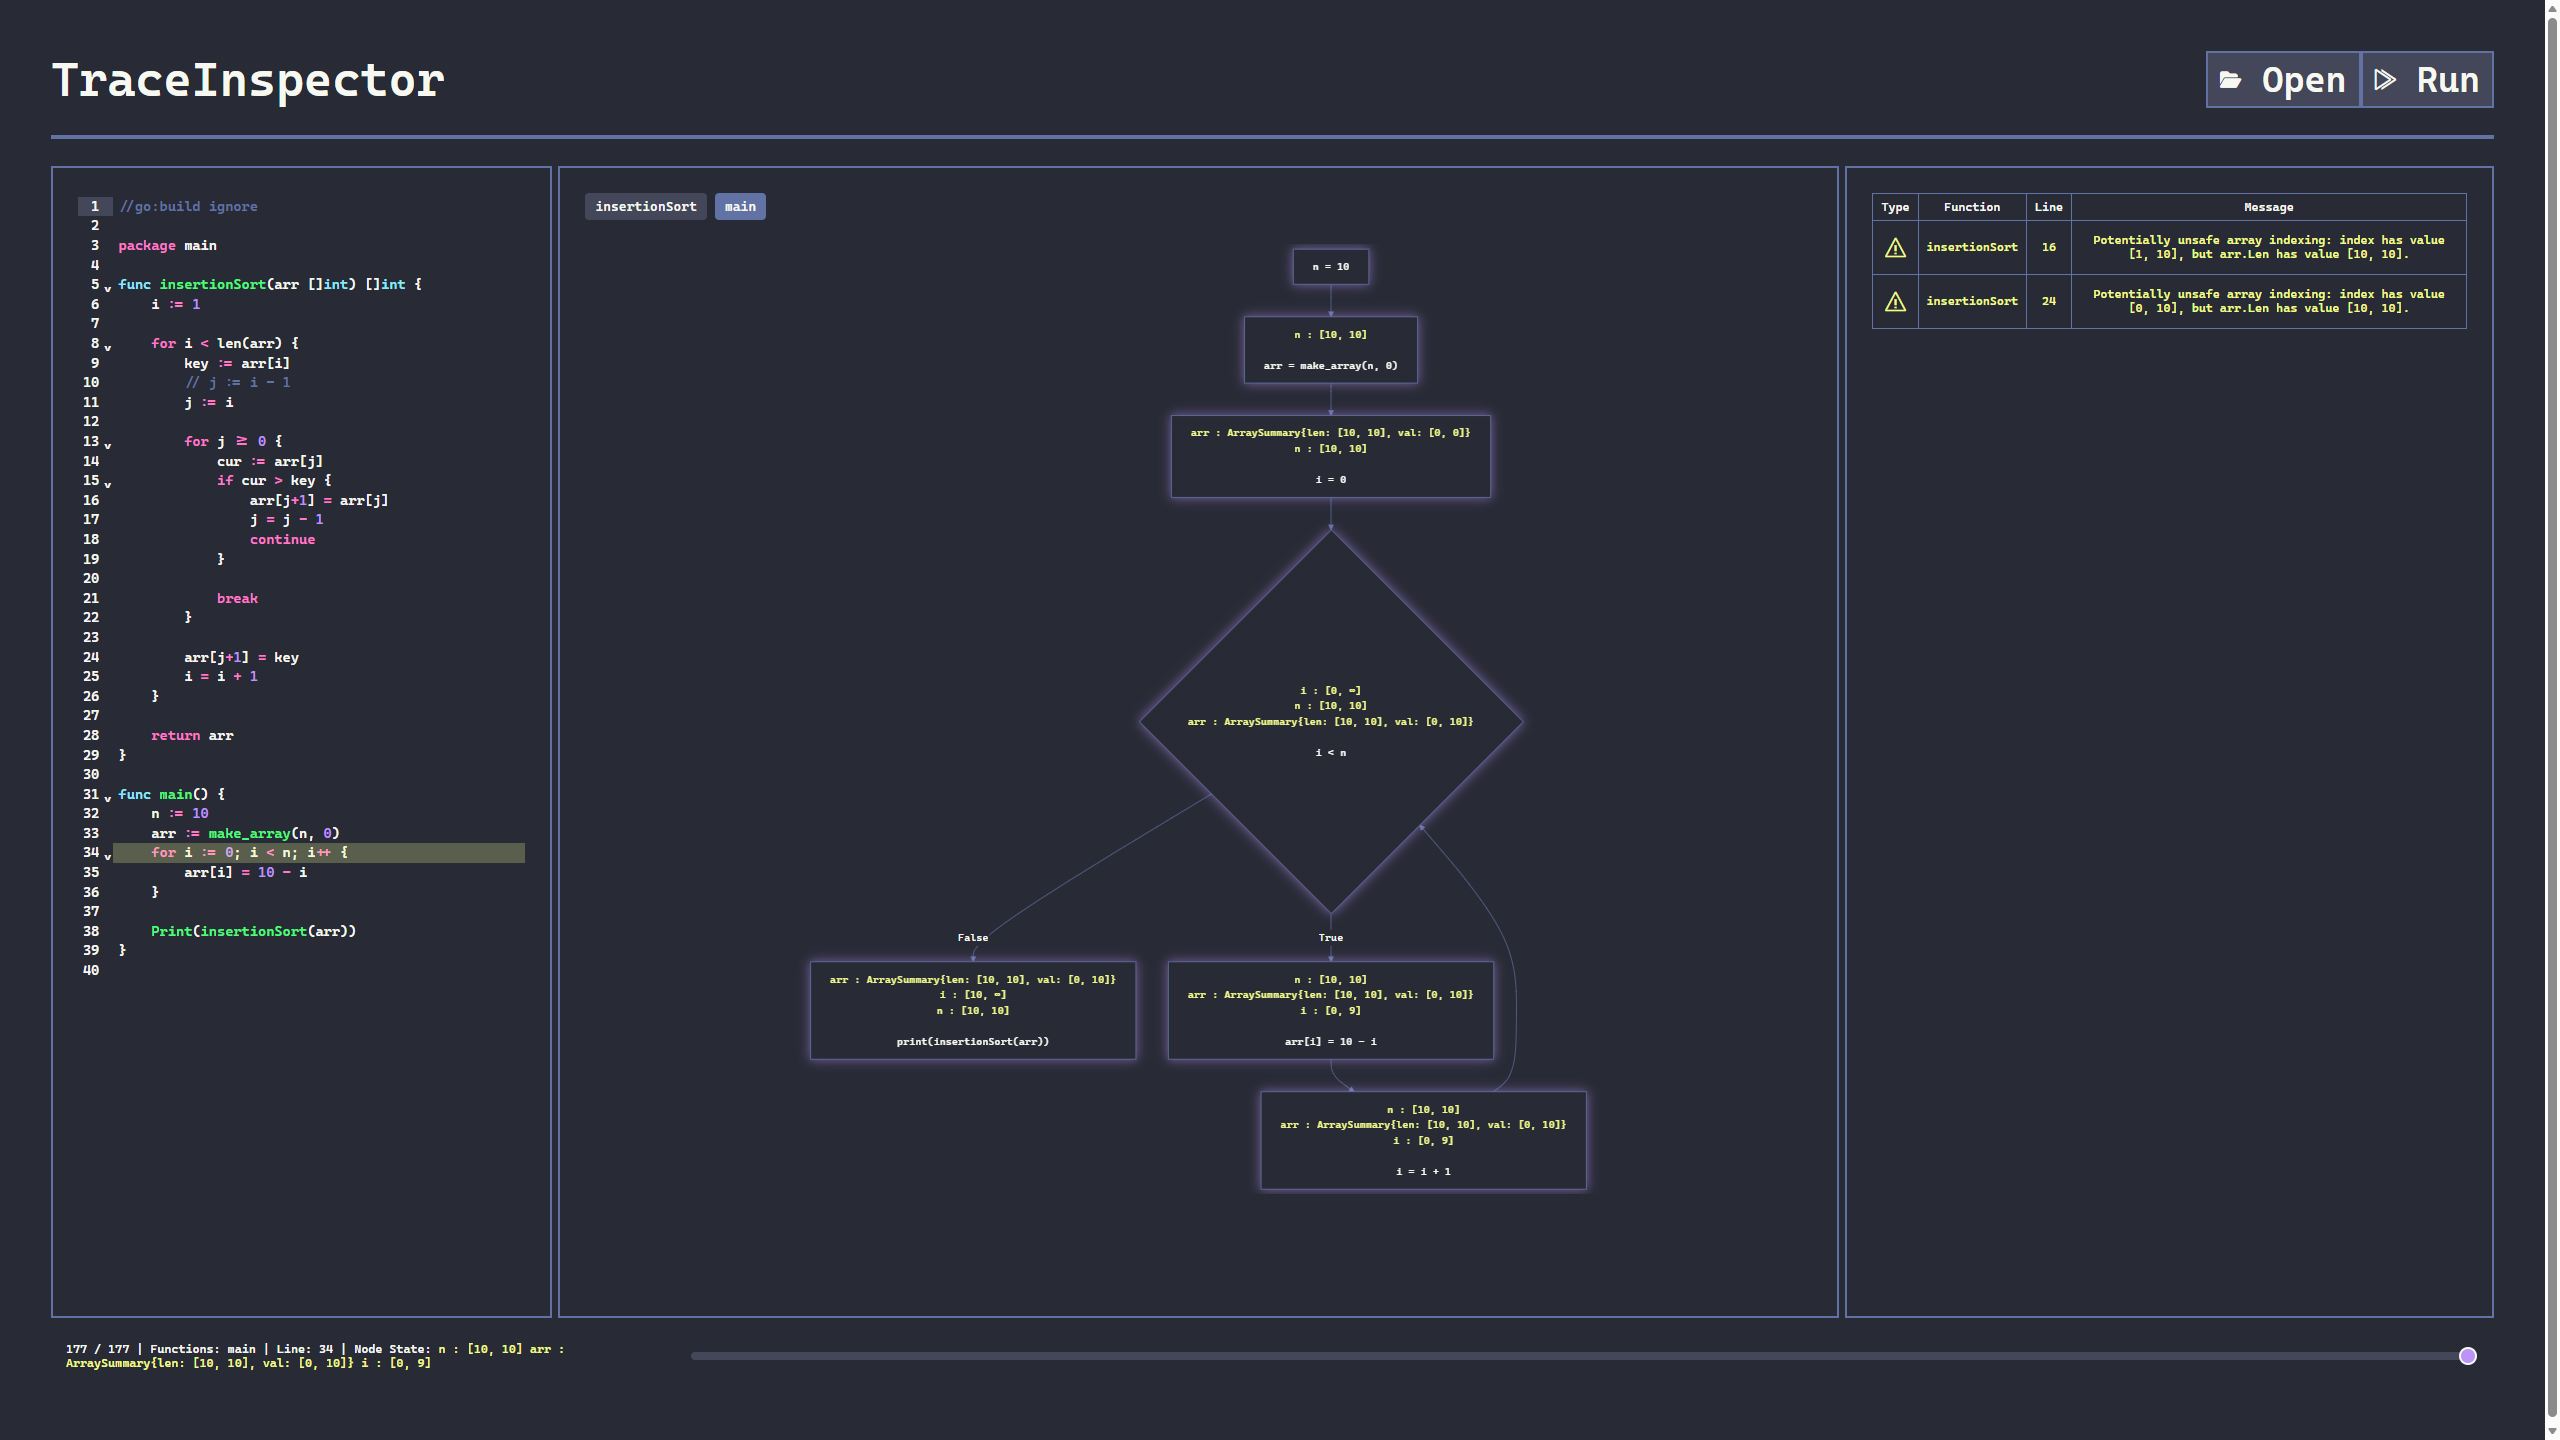
\includegraphics[width=\linewidth, height=14cm, keepaspectratio]{images/Inspector.png}%
            \end{center}
        \end{minipage}
        \begin{minipage}{0.25\textwidth}
            하단 슬라이더를 통해 프로그램 실행 상태 변화를 관찰할 수 있음.
        \end{minipage}
\end{bpbox}
\begin{bpbox}[bpcolor=grey, bpstyle=wide, title={한계 및 향후 계획}]
    \begin{itemize}
        \item 관계형 요약도메인 : \texttt{i < len(arr)} 등과 같이 구체적인 값이 아닌 변수간의 논리적 관계를 나태닐 수 있는 대수적 도메인.
        \item Divide by zero, unreachable code등 보다 다양한 오류 탐지.
        \item Pointer inference : 포인터 및 메모리 동작 추상화를 통한 liveness 성질 검증.
        \item \inleq{\mathsf{C} \rightarrow \mathsf{Imp}, \mathsf{Rust} \rightarrow \mathsf{Imp}} 등 \inleq{\mathsf{Imp}}를 활용한 다양한 언어 지원.
        \item 보다 다양한 언어 기능 지원 : 확장된 타입 체계, widening 휴리스틱 등
    \end{itemize}
\end{bpbox}
\end{bpcolumns}

\end{document}